\documentclass[11pt]{beamer}
\usepackage[utf8]{inputenc}
\usepackage[T1]{fontenc}
\usepackage{lmodern}
\usepackage[english]{babel}
\usepackage{booktabs}
\usepackage{fontawesome}
\usetheme{Darmstadt}
\setbeamertemplate{navigation symbols}{}
\setbeamertemplate{footline}{
	\begin{beamercolorbox}[ht=3ex,leftskip=1.4cm,rightskip=.3cm]{author in head/foot}
		\hfill \insertframenumber
		\vspace*{0.07cm}
	\end{beamercolorbox}
} 
\usepackage{url}
\usepackage{hyperref}

% color def
\usepackage{color}
\definecolor{darkred}{rgb}{0.6,0.0,0.0}
\definecolor{darkgreen}{rgb}{0,0.50,0}
\definecolor{lightblue}{rgb}{0.0,0.42,0.91}
\definecolor{orange}{rgb}{0.99,0.48,0.13}
\definecolor{grass}{rgb}{0.18,0.80,0.18}
\definecolor{pink}{rgb}{0.97,0.15,0.45}

\usepackage{listings}
\usepackage{upquote}


\newcommand\Wider[2][3em]{%
\makebox[\linewidth][c]{%
  \begin{minipage}{\dimexpr\textwidth+#1\relax}
  \raggedright#2
  \end{minipage}%
  }%
}

\lstdefinestyle{Python}{
    language=Python,
    morekeywords=[1]{,as,assert,nonlocal,with,yield,self,True,False,None,} % Python builtin
	morekeywords=[2]{,__init__,__add__,__mul__,__div__,__sub__,__call__,__getitem__,__setitem__,__eq__,__ne__,__nonzero__,__rmul__,__radd__,__repr__,__str__,__get__,__truediv__,__pow__,__name__,__future__,__all__,}, % magic methods
	morekeywords=[3]{,object,type,isinstance,copy,deepcopy,zip,enumerate,reversed,list,set,len,dict,tuple,range,xrange,append,execfile,real,imag,reduce,str,repr,}, % common functions
	morekeywords=[4]{,Exception,NameError,IndexError,SyntaxError,TypeError,ValueError,OverflowError,ZeroDivisionError,}, % errors
	morekeywords=[5]{,ode,fsolve,sqrt,exp,sin,cos,arctan,arctan2,arccos,pi, array,norm,solve,dot,arange,isscalar,max,sum,flatten,shape,reshape,find,any,all,abs,plot,linspace,legend,quad,polyval,polyfit,hstack,concatenate,vstack,column_stack,empty,zeros,ones,rand,vander,grid,pcolor,eig,eigs,eigvals,svd,qr,tan,det,logspace,roll,min,mean,cumsum,cumprod,diff,vectorize,lstsq,cla,eye,xlabel,ylabel,squeeze,}, % numpy / math
	%morestring=*[b]{"},
    basicstyle=\ttfamily,
   	backgroundcolor=\color{white},
   	commentstyle=\color{darkgreen}\slshape,
   	keywordstyle=\color{blue}\bfseries\itshape,
   	keywordstyle=[2]\color{blue}\bfseries,
   	keywordstyle=[3]\color{grass},
   	keywordstyle=[4]\color{red},
   	keywordstyle=[5]\color{orange},
   	stringstyle=\color{darkred},
   	emphstyle=\color{pink}\underbar,
    % honek neretako bakarrik die
    %deletekeywords=[2]{next,set},
    %deletekeywords=[3]{next,set},
}

% General Setting of listings
\lstset{
    style=Python,
	tabsize=4,
	aboveskip=1em,
	breaklines=true,
	abovecaptionskip=-6pt,
	captionpos=b,
	escapeinside={\%*}{*)},
	frame=single,
	numbers=left,
	numbersep=8pt,
	numberstyle=\tiny,
    showstringspaces=false,
}

\definecolor{delim}{RGB}{20,105,176}
\definecolor{numb}{RGB}{106, 109, 32}
\definecolor{string}{rgb}{0.64,0.08,0.08}

\lstdefinelanguage{json}{
    showspaces=false,
    showtabs=false,
    breaklines=true,
    postbreak=\raisebox{0ex}[0ex][0ex]{\ensuremath{\color{gray}\hookrightarrow\space}},
    breakatwhitespace=true,
    basicstyle=\ttfamily\small,
    upquote=true,
    morestring=[b]",
    stringstyle=\color{string},
    literate=
     *{0}{{{\color{numb}0}}}{1}
      {1}{{{\color{numb}1}}}{1}
      {2}{{{\color{numb}2}}}{1}
      {3}{{{\color{numb}3}}}{1}
      {4}{{{\color{numb}4}}}{1}
      {5}{{{\color{numb}5}}}{1}
      {6}{{{\color{numb}6}}}{1}
      {7}{{{\color{numb}7}}}{1}
      {8}{{{\color{numb}8}}}{1}
      {9}{{{\color{numb}9}}}{1}
      {\{}{{{\color{delim}{\{}}}}{1}
      {\}}{{{\color{delim}{\}}}}}{1}
      {[}{{{\color{delim}{[}}}}{1}
      {]}{{{\color{delim}{]}}}}{1},
}

\usepackage{tikz}
\usetikzlibrary{calc,shapes.multipart,chains,arrows,positioning}
\usetikzlibrary {shapes.misc} 
\usetikzlibrary{shadows.blur}
\usetikzlibrary{matrix}
\tikzset{
stack_item/.style={rounded rectangle, rounded rectangle arc length=90,draw, anchor=center, fill=white, minimum width=2cm, minimum height=0.7cm},
bar/.style={rounded rectangle, minimum width=3cm, fill=black, blur shadow={shadow blur steps=5,shadow blur extra rounding=1.3pt}},
message/.style={rectangle, fill=white, color=white, text=black},
bowling_pin/.style={circle, draw, line width=0.6mm, color=red, text=black, minimum width=8mm},
empty/.style={circle, draw, line width=0.6mm, color=white, text=black, minimum width=8mm},
table_cell/.style={rectangle, draw, color=black, text=black, minimum size=12mm}
}

\tikzset{
	squarecross/.style={
		draw, rectangle,minimum size=18pt, fill=orange!80,
		inner sep=0pt, text=black,
		path picture = {
			\draw[-,black]
			(path picture bounding box.north west) --
			(path picture bounding box.south east)
			(path picture bounding box.south west) --
			(path picture bounding box.north east);
		}
	},
	list/.style={
		very thick, rectangle split,
		rectangle split parts=2, draw,
		rectangle split horizontal, minimum size=18pt,
		inner sep=4pt, text=black,
		rectangle split part fill={red!20, blue!20}
	},
	->, start chain, very thick,
	chain_arrow/.style={*->, thick}
}

\usetikzlibrary{arrows.meta}
\tikzset{
    queue element/.style={
        draw,very thin,rounded corners,
        fill=white,
        minimum width=1cm,minimum height=.5cm,
        font=\sffamily\footnotesize
    },
    >={[scale=0.8]Triangle}
}

\author{Estructura de Datos}
\title{\huge{Pilas y Colas}}
\titlegraphic{
\includegraphics[width=3cm]{img/UPNA}}
\date[]{2024-2025}
\subject{Estructura de Datos}
%\subtitle{}
%\logo{}
%\institute{}
%\date{}
%\subject{}
%\setbeamercovered{transparent}
%\setbeamertemplate{navigation symbols}{}

\AtBeginSection[]{
	\begin{frame}[plain]
		\frametitle{}
		\tableofcontents[currentsection, hideothersubsections]
	\end{frame}
}

\begin{document}
\begin{frame}[plain]
	\maketitle
\end{frame}

\begin{frame}
	\tableofcontents
\end{frame}

\section{Tipos Abstractos de Datos}

\begin{frame}\frametitle{¿Qué es un \textit{TAD}?}
\begin{itemize}
\item Un \textit{Tipo Abstracto de Datos} (TAD) es una forma de modelar la interacción que un usuario tiene con los datos
\item La estructura se define solo conceptualmente
    \begin{itemize}
    \item Valores posibles
    \item Operaciones sobre el tipo de datos y su comportamiento
    \end{itemize}
\item Un TAD describe la forma lógica de los datos, una \textbf{estructura de datos} es su implementación
\end{itemize}
\end{frame}

\section{\textit{TADs} implementados en Python}

\begin{frame}\frametitle{Algunos TADs ya están implementados en Python}
\begin{itemize}
\item La mayoría de los lenguajes de programación ya implementan algunos TADs
\item Python tiene varios en las bibliotecas principales:
    \begin{itemize}
    \item Listas
    \item Mapas (Diccionarios)
    \item Conjuntos
    \end{itemize}
\item Hay más en bibliotecas externas
    \begin{itemize}
    \item Colas/Deques
    \item Árboles
    \item Grafos
    \end{itemize}
\end{itemize}
\end{frame}

\subsection{Listas}

\begin{frame}\frametitle{El TAD Lista}
\begin{itemize}
\item La \texttt{Lista} es uno de los TAD más comunes
\item Almacena puntos de datos en un orden dado
    \begin{itemize}
    \item La longitud de la lista suele ser dinámica
    \end{itemize}
\item Métodos básicos de \texttt{Lista}
    \begin{itemize}
    \item Crear una lista vacía
    \item Comprobar si la lista está vacía
    \item Añadir un elemento a la lista
    \item Eliminar un elemento de la lista
    \item Acceder a un elemento con un índice
    \end{itemize}
\end{itemize}
\vspace{0.4cm}
\begin{center}
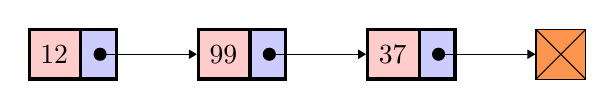
\begin{tikzpicture}
  \node[list,on chain] (A) {12};
  \node[list,on chain] (B) {99};
  \node[list,on chain] (C) {37};
  \node[squarecross]   (D) [right=of C] {};
  \draw[*->] let \p1 = (A.two), \p2 = (A.center) in (\x1,\y2) -- (B);
  \draw[*->] let \p1 = (B.two), \p2 = (B.center) in (\x1,\y2) -- (C);
  \draw[*->] let \p1 = (C.two), \p2 = (C.center) in (\x1,\y2) -- (D);
\end{tikzpicture}
\end{center}
\end{frame}

\begin{frame}\frametitle{Listas en Python}

\Wider{\centering\scriptsize
\begin{tabular}{@{}lll@{}}
\toprule
\textbf{Método} & \textbf{Uso} & \textbf{Explicación} \\
\midrule
\texttt{append} & \texttt{a\_list.append(item)} & Añade un nuevo elemento al final de una lista \\
\texttt{insert} & \texttt{a\_list.insert(i, item)} & Inserta un elemento en la posición $i^{th}$ de una lista \\
\texttt{pop} & \texttt{a\_list.pop()} & Elimina y devuelve el último elemento de una lista \\
\texttt{pop} & \texttt{a\_list.pop(i)} & Elimina y devuelve el elemento $i^{th}$ de una lista \\
\texttt{sort} & \texttt{a\_list.sort()} & Modifica una lista para que esté ordenada \\
\texttt{reverse} & \texttt{a\_list.reverse()} & Modifica una lista para que esté en orden inverso \\
\texttt{\textbf{del}} & \texttt{\textbf{del} a\_list[i]} & Elimina el elemento en la posición $i^{th}$ \\
\texttt{index} & \texttt{a\_list.index(item)} & Devuelve el índice de la primera aparición del elemento \\
\texttt{count} & \texttt{a\_list.count(item)} & Devuelve el número de apariciones del elemento \\
\texttt{remove} & \texttt{a\_list.remove(item)} & Elimina la primera aparición del elemento \\
\bottomrule
\end{tabular}
}
\vspace{0.4cm}
\begin{block}{Más información}
\href{https://docs.python.org/3/tutorial/datastructures.html}{\color{blue}\underline{https://docs.python.org/3/tutorial/datastructures.html}}
\end{block}
\end{frame}

\subsection{Mapas}

\begin{frame}\frametitle{El TAD Mapa}
\begin{itemize}
\item Un \texttt{Mapa} es una colección de pares $<clave, valor>$
\item Puede ser implementado usando tablas hash, árboles de búsqueda u otras estructuras
\item Métodos básicos de \texttt{Mapa}:
    \begin{itemize}
    \item Insertar un nuevo par $<clave, valor>$
    \item Eliminar un par $<clave, valor>$
    \item Obtener un valor a partir de una clave dada
    \end{itemize}
\end{itemize}
\end{frame}

\begin{frame}\frametitle{Mapas en Python}
\Wider{\centering\scriptsize
\begin{tabular}{@{}lll@{}}
\toprule
\textbf{Método} & \textbf{Uso} & \textbf{Explicación} \\
\midrule
 & \texttt{a\_dict[key] = value} & Establece un valor para una clave \\
 & \texttt{a\_dict[key]} & Devuelve el valor asociado con la clave \\
\texttt{keys} & \texttt{a\_dict.keys()} & Devuelve las claves del diccionario en un objeto \texttt{dict\_keys} \\
\texttt{values} & \texttt{a\_dict.values()} & Devuelve las claves del diccionario en un objeto \texttt{dict\_values} \\
\texttt{items} & \texttt{a\_list.items} & Devuelve los pares clave-valor en un objeto \texttt{dict\_items} \\
\texttt{get} & \texttt{a\_list.get(key)} & Devuelve el valor asociado con \texttt{key}, \texttt{None} en caso contrario \\
\texttt{get} & \texttt{a\_list.get(key, alt)} & Devuelve el valor asociado con \texttt{key}, \texttt{alt} en caso contrario \\
\bottomrule
\end{tabular}
\normalsize
\vspace{0.4cm}

\begin{block}{Más información}
\href{https://docs.python.org/3/tutorial/datastructures.html\#dictionaries}{\color{blue}\underline{https://docs.python.org/3/tutorial/datastructures.html\#dictionaries}}
\end{block}
}
\end{frame}

\section{Pila}

\begin{frame}\frametitle{El TAD Pila}
\begin{itemize}
\item Último en entrar, primero en salir (LIFO, por sus siglas en inglés)
\end{itemize}
\vspace{0.4cm}
\begin{center}
\scalebox{1.5}{
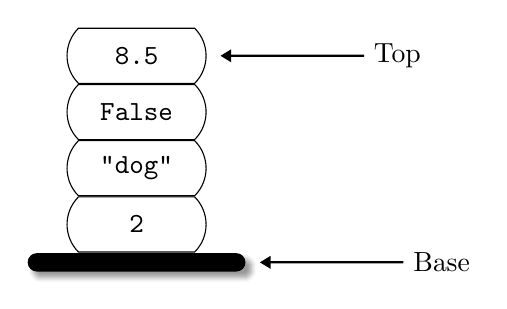
\begin{tikzpicture}
    \node[bar] (base_1) {};
    \node[stack_item] (1_1) [above=0 of base_1] {\texttt{2}};
    \node[stack_item] (1_2) [above=0 of 1_1] {\texttt{"dog"}};
    \node[stack_item] (1_3) [above=0 of 1_2] {\texttt{False}};
    \node[stack_item] (1_4) [above=0 of 1_3] {\texttt{8.5}};
    \node (base) [right=2cm of base_1] {Base};
    \node (text) [right=2cm of 1_4] {Top};
    \draw[->, shorten >=5pt, thick] (base) -- (base_1);
    \draw[->, shorten >=5pt, thick] (text) -- (1_4);
\end{tikzpicture}
}
\end{center}
\end{frame}

\begin{frame}\frametitle{Operaciones en una Pila}
\begin{itemize}
\item La Pila tendrá al menos dos operaciones
    \begin{description}
    \item[push:] Añadir un nuevo elemento en la parte superior de la Pila
    \item[pop:] Eliminar y devolver el elemento superior de la Pila
    \end{description}
\item Puede haber más operaciones opcionales
    \begin{description}
    \item[peek:] Devolver el elemento superior de la Pila sin eliminarlo
    \item[is\_empty:] Devuelve \lstinline|True| si la Pila está vacía, \lstinline|False| en caso contrario
    \item[size:] Devuelve el número de elementos en la Pila
    \end{description}
\end{itemize}
\end{frame}

\begin{frame}\frametitle{La <operación \texttt{push} I}
\begin{center}
\scalebox{1.5}{
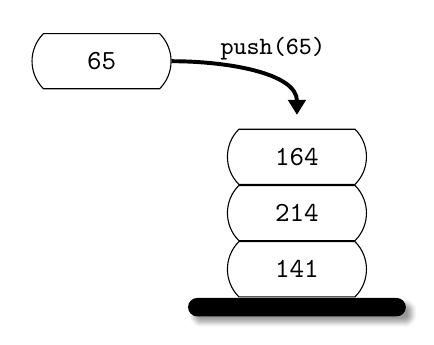
\begin{tikzpicture}
    \node[bar] (base_1) {};
    \node[stack_item] (1_1) [above=0 of base_1] {\texttt{141}};
    \node[stack_item] (1_2) [above=0 of 1_1] {\texttt{214}};
    \node[stack_item] (1_3) [above=0 of 1_2] {\texttt{164}};
    \node[stack_item] (1_4) [above left=0.5 and 1 of 1_3] {\texttt{65}};
    \draw[->, shorten >=5pt, line width=0.5mm] (1_4.east) to [out=0,in=90] (1_3.north) node[midway, above left=3cm and -0.5cm] {\small\texttt{push(65)}};
\end{tikzpicture}
}
\end{center}
\end{frame}

\begin{frame}\frametitle{La <operación \texttt{push} II}
\begin{center}
\scalebox{1.5}{
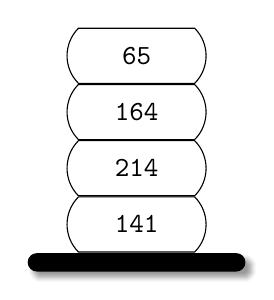
\begin{tikzpicture}
    \node[bar] (base_1) {};
    \node[stack_item] (1_1) [above=0 of base_1] {\texttt{141}};
    \node[stack_item] (1_2) [above=0 of 1_1] {\texttt{214}};
    \node[stack_item] (1_3) [above=0 of 1_2] {\texttt{164}};
    \node[stack_item] (1_4) [above=0 of 1_3] {\texttt{65}};
\end{tikzpicture}
}
\end{center}
\end{frame}

\begin{frame}\frametitle{La <operación \texttt{pop} I}
\begin{center}
\scalebox{1.5}{
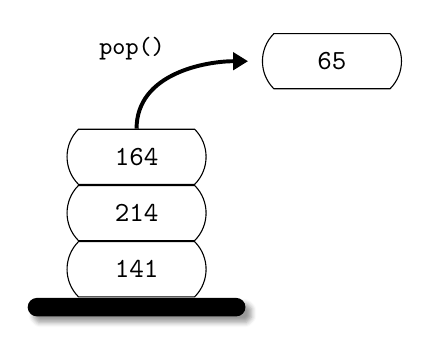
\begin{tikzpicture}
    \node[bar] (base_1) {};
    \node[stack_item] (1_1) [above=0 of base_1] {\texttt{141}};
    \node[stack_item] (1_2) [above=0 of 1_1] {\texttt{214}};
    \node[stack_item] (1_3) [above=0 of 1_2] {\texttt{164}};
    \node[stack_item] (1_4) [above right=0.5 and 1 of 1_3] {\texttt{65}};
    \draw[->, shorten >=5pt, line width=0.5mm] (1_3.north) to [out=90,in=180] (1_4.west) node[midway, above left=3cm and -0.5cm] {\small\texttt{pop()}};
\end{tikzpicture}
}
\end{center}
\end{frame}

\begin{frame}\frametitle{La <operación \texttt{pop} II}
\begin{center}
\scalebox{1.5}{
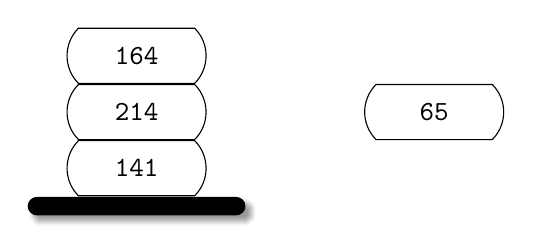
\begin{tikzpicture}
    \node[bar] (base_1) {};
    \node[stack_item] (1_1) [above=0 of base_1] {\texttt{141}};
    \node[stack_item] (1_2) [above=0 of 1_1] {\texttt{214}};
    \node[stack_item] (1_3) [above=0 of 1_2] {\texttt{164}};
    \node[stack_item] (1_4) [right=2 of 1_2] {\texttt{65}};
\end{tikzpicture}
}
\end{center}
\end{frame}

\begin{frame}\frametitle{La <operación \texttt{peek} I}
\begin{center}
\scalebox{1.5}{
\begin{tikzpicture}
    \node[bar] (base_1) {};
    \node[stack_item] (1_1) [above=0 of base_1] {\texttt{141}};
    \node[stack_item] (1_2) [above=0 of 1_1] {\texttt{214}};
    \node[stack_item] (1_3) [above=0 of 1_2] {\texttt{164}};
    \node[stack_item] (1_4) [above=0 of 1_3] {\texttt{65}};
    \node (eye) [left=1.5 of 1_4] {\Huge\faEye};
    \draw[->, shorten >=5pt, line width=0.5mm] (eye) to (1_4) node[midway, above left=2.6cm and 1cm] {\small\texttt{peek()}};
\end{tikzpicture}
}
\end{center}
\end{frame}

\begin{frame}\frametitle{La <operación \texttt{peek} II}
\begin{center}
\scalebox{1.5}{
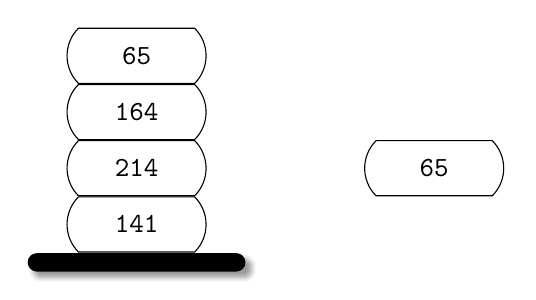
\begin{tikzpicture}
    \node[bar] (base_1) {};
    \node[stack_item] (1_1) [above=0 of base_1] {\texttt{141}};
    \node[stack_item] (1_2) [above=0 of 1_1] {\texttt{214}};
    \node[stack_item] (1_3) [above=0 of 1_2] {\texttt{164}};
    \node[stack_item] (1_4) [above=0 of 1_3] {\texttt{65}};
    \node[stack_item] (1_5) [right=2 of 1_2] {\texttt{65}};
\end{tikzpicture}
}
\end{center}
\end{frame}

\begin{frame}\frametitle{Creación de una Pila}
\begin{block}{}
\centering\Huge ¿Cómo crearías una Pila usando Python?
\end{block}
\end{frame}


\section{Cola}

\begin{frame}\frametitle{El TAD Cola}
\begin{itemize}
\item Primero en entrar, primero en salir (FIFO, por sus siglas en inglés)
\end{itemize}
\vspace{0.4cm}
\begin{center}
\scalebox{1.5}{
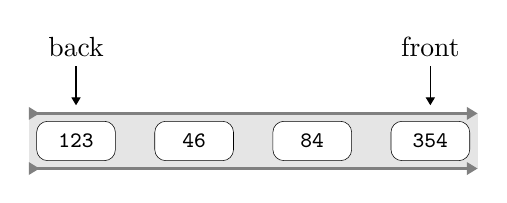
\begin{tikzpicture}
\fill[gray!20] (5.1,.35) rectangle (-.6,-.35);
\draw[gray,thick,>->] (-.6,.35) -- (5.1,.35);
\draw[gray,thick,>->] (-.6,-.35) -- (5.1,-.35);
\foreach \i/\name in {0/123,1/46,2/84,3/354}
    \node[queue element] (elem_\i) at (1.5*\i,0) {\texttt{\name}};
\draw[<-] ([yshift=.2cm]elem_3.north) -- ++ (0,.5) node[above] {front};
\draw[<-] ([yshift=.2cm]elem_0.north) -- ++ (0,.5) node[above] {back};
\end{tikzpicture}
}
\end{center}
\end{frame}

\begin{frame}\frametitle{Operaciones en una Cola}
\begin{itemize}
\item La Cola tendrá al menos dos operaciones
    \begin{description}
    \item[enqueue:] Añadir un nuevo elemento al final de la Cola
    \item[dequeue:] Eliminar y devolver un elemento del frente de la Cola
    \end{description}
\item Al igual que con las Pilas, una Cola puede tener más operaciones
    \begin{description}
    \item[peek:] Devolver el elemento frontal de la Cola sin eliminarlo
    \item[is\_empty:] Devuelve \lstinline|True| si la Cola está vacía, \lstinline|False| en caso contrario
    \item[size:] Devuelve el número de elementos en la Cola
    \end{description}
\end{itemize}
\end{frame}

\begin{frame}\frametitle{La operación \texttt{enqueue} I}

\begin{center}
\scalebox{1.5}{
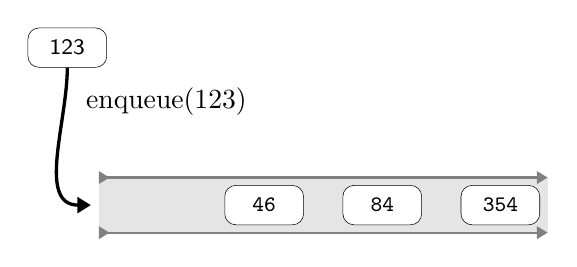
\begin{tikzpicture}
\fill[gray!20] (5.1,.35) rectangle (-.6,-.35);
\draw[gray,thick,>->] (-.6,.35) -- (5.1,.35);
\draw[gray,thick,>->] (-.6,-.35) -- (5.1,-.35);
\foreach \i/\name in {1/46,2/84,3/354}
    \node[queue element] (elem_\i) at (1.5*\i,0) {\texttt{\name}};
\node[queue element] (0) at (-1,2) {123};
\draw[->,very thick] (0.south) to[out=-90,in=180] (-.7,0) node[midway, above right=1 and -0.9] {enqueue(123)};
\end{tikzpicture}
}
\end{center}
\end{frame}

\begin{frame}\frametitle{La operación \texttt{enqueue} II}
\begin{center}
\scalebox{1.5}{
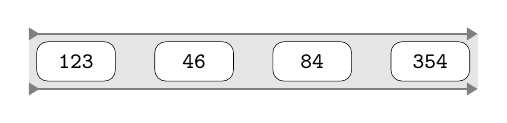
\begin{tikzpicture}
\fill[gray!20] (5.1,.35) rectangle (-.6,-.35);
\draw[gray,thick,>->] (-.6,.35) -- (5.1,.35);
\draw[gray,thick,>->] (-.6,-.35) -- (5.1,-.35);
\foreach \i/\name in {0/123,1/46,2/84,3/354}
    \node[queue element] (elem_\i) at (1.5*\i,0) {\texttt{\name}};
\end{tikzpicture}
}
\end{center}
\end{frame}


\begin{frame}\frametitle{La operación \texttt{dequeue} I}
\begin{center}
\scalebox{1.5}{
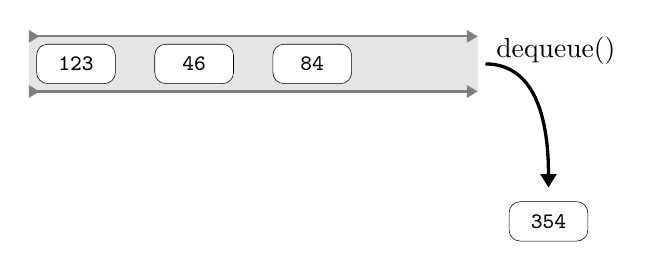
\begin{tikzpicture}
\fill[gray!20] (5.1,.35) rectangle (-.6,-.35);
\draw[gray,thick,>->] (-.6,.35) -- (5.1,.35);
\draw[gray,thick,>->] (-.6,-.35) -- (5.1,-.35);
\foreach \i/\name in {0/123,1/46,2/84}
    \node[queue element] (elem_\i) at (1.5*\i,0) {\texttt{\name}};
\node[queue element] (3) at (6,-2) {\texttt{354}};
\draw[->,very thick, shorten >=5pt] (5.2,0) to[out=0,in=90] (3.north) node[above right=1.6 and -0.8] {dequeue()};
\end{tikzpicture}
}
\end{center}
\end{frame}


\begin{frame}\frametitle{La operación \texttt{dequeue} I}
\begin{center}
\scalebox{1.5}{
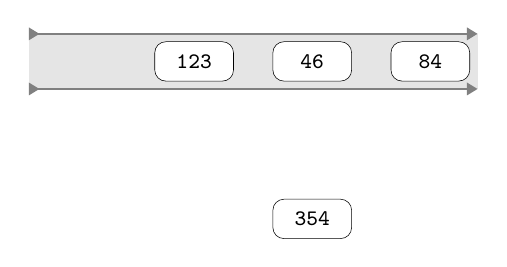
\begin{tikzpicture}
\fill[gray!20] (5.1,.35) rectangle (-.6,-.35);
\draw[gray,thick,>->] (-.6,.35) -- (5.1,.35);
\draw[gray,thick,>->] (-.6,-.35) -- (5.1,-.35);
\foreach \i/\name in {1/123,2/46,3/84}
    \node[queue element] (elem_\i) at (1.5*\i,0) {\texttt{\name}};
\node[queue element] (4) at (3,-2) {\texttt{354}};
\end{tikzpicture}
}
\end{center}
\end{frame}

\begin{frame}\frametitle{La operación \texttt{peek} I}
\begin{center}
\scalebox{1.5}{
\begin{tikzpicture}
\fill[gray!20] (5.1,.35) rectangle (-.6,-.35);
\draw[gray,thick,>->] (-.6,.35) -- (5.1,.35);
\draw[gray,thick,>->] (-.6,-.35) -- (5.1,-.35);
\foreach \i/\name in {0/123,1/46,2/84,3/354}
    \node[queue element] (elem_\i) at (1.5*\i,0) {\texttt{\name}};
\node (eye) [above=1.5 of elem_3] {\Huge\faEye};
\draw[->, shorten >=5pt, line width=0.5mm] (eye) to (elem_3) node[above right=1cm and 0cm] {\small\texttt{peek()}};
\end{tikzpicture}
}
\end{center}
\end{frame}

\begin{frame}\frametitle{La operación \texttt{peek} II}
\begin{center}
\scalebox{1.5}{
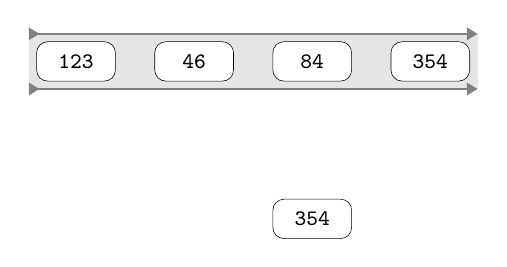
\begin{tikzpicture}
\fill[gray!20] (5.1,.35) rectangle (-.6,-.35);
\draw[gray,thick,>->] (-.6,.35) -- (5.1,.35);
\draw[gray,thick,>->] (-.6,-.35) -- (5.1,-.35);
\foreach \i/\name in {0/123,1/46,2/84,3/354}
    \node[queue element] (elem_\i) at (1.5*\i,0) {\texttt{\name}};
\node[queue element] (4) at (3,-2) {\texttt{354}};
\end{tikzpicture}
}
\end{center}
\end{frame}

\begin{frame}\frametitle{Creación de una Cola}
\begin{block}{}
\centering\Huge ¿Cómo crearías una Cola usando Python?
\end{block}
\end{frame}


%\section{JSON}
%
%\begin{frame}\frametitle{What is JSON}
%\begin{itemize}
%\item Oringinated from JavaScript $\rightarrow$ JavaScript Object Notation
%    \begin{itemize}
%    \item Language-independent
%    \item Many modern languages have support to generate or parse it
%    \end{itemize}
%\item A standard for data interchange using human-readable text
%    \begin{itemize}
%    \item An alternative to XML
%    \end{itemize}
%\item Data is stored in $<attribute,value>$ pairs
%    \begin{itemize}
%    \item Similar to a dictionary in Python
%    \end{itemize}
%\end{itemize}
%\end{frame}
%
%
%\begin{frame}[fragile]\frametitle{JSON example}
%\begin{lstlisting}[basicstyle=\ttfamily\tiny,numberstyle=\tiny]
%{
%  "first_name": "John",
%  "last_name": "Smith",
%  "is_alive": true,
%  "age": 27,
%  "address": {
%    "street_address": "21 2nd Street",
%    "city": "New York",
%    "state": "NY",
%    "postal_code": "10021-3100"
%  },
%  "phone_numbers": [
%    {
%      "type": "home",
%      "number": "212 555-1234"
%    },
%    {
%      "type": "office",
%      "number": "646 555-4567"
%    }
%  ]
%}
%\end{lstlisting}
%\end{frame}
%
%\begin{frame}\frametitle{JSON Data Types}
%\begin{description}
%\item[Object:] The $<key, value>$ pairs, similar to a \lstinline|dict|
%\item[Number:] A number, similar to a \lstinline|float|
%\item[String:] A sequence of characters delimited by double quotes
%\item[Boolean:] A \lstinline|true| or \lstinline|false| value
%\item[Array:] A ordered list of elements, similar to \lstinline|list|
%\item[null:] An empty value, similar to \lstinline|None|
%\end{description}
%\end{frame}
%
%\begin{frame}\frametitle{Webpages to Play with JSON}
%\begin{itemize}
%\setlength\itemsep{0.4cm}
%\item \href{http://www.json.org/json-en.html}{\color{blue}\underline{http://www.json.org/json-en.html}}
%\item \href{https://codebeautify.org/jsonviewer}{\color{blue}\underline{https://codebeautify.org/jsonviewer}}
%\item \href{http://jsonviewer.stack.hu/}{\color{blue}\underline{http://jsonviewer.stack.hu/}}
%\end{itemize}
%\end{frame}



\end{document}